%% using aastex version 6.2
\documentclass[twocolumn, dvipdfmx]{aastex62}
\usepackage{CJK}
\usepackage{textcomp}
\usepackage{graphicx}
\usepackage{here}
\usepackage{hhline}
\usepackage{longtable}

\def\red<#1>{\textcolor{red}{#1}}
\newcommand\aastex{AAS\TeX}
\newcommand\latex{La\TeX}

\received{\today}
\revised{\today}
\accepted{\today}
\submitjournal{ApJ}

\shortauthors{Goda \& Matsuo}

\begin{document}
\begin{CJK*}{UTF8}{min}

\title{Multiple populations of extrasolar gas giants}

\author{Shohei Goda}
\affil{\rm Department of Earth and Space Science, Graduate School of Science, Osaka University, 1-1, Machikaneyamacho, Toyonaka, Osaka 560-0043, Japan}

\author{Taro Matsuo}
\affiliation{\rm Department of Earth and Space Science, Graduate School of Science, Osaka University, 1-1, Machikaneyamacho, Toyonaka, Osaka 560-0043, Japan}


\begin{abstract}

Statistically verifying the character of exoplanets, we can expect to reveal the formation or evolution processes of planetary systems. The notable parameters of planetary systems are metallicity of host star, planet mass, and eccentricity. Gas giants around metal rich stars are easily formed by core accretion. Since these planets are grown with bottom up, the distributions of planet masses and eccentricities are seemed to be continuously extended.
On the other hand, the planetary formation by disk instability depends on mass and effective temperature of protoplanetary disk, but there is no strongly dependence on metallicity of host star. As these planets are not formed with bottom up, the planetary masses and eccentricities ununiformly distribute. In this study, we statistically revealed the planetary distributions of metal-rich and -poor regions, and tried to understand the planetary-formation and -evolution processes. Note that we made the dataset included the both selection biases of planetary detection for metal-rich and -poor regions to ignore the effect of these biases. As the results from classification for those samples with Gaussian Mixture Model, we found that the planetary distribution was divided into 3 regions by the boundaries around 3 and 13 $\rm M_J$. We also discovered the different distributions of planet mass between each metallicity region, which explains the different processes of the planetary formation: core accretion model is applied in metal-rich region, and several formation models including core accretion are match in metal-poor region. In addition, we found that the distributions of planetary eccentricity have a difference between each mass cluster, especially in metal-rich region, which implies that there are dynamical interactions after the planets formed by core accretion.


\end{abstract}

\vspace{1cm}

\keywords{methods: data analysis -- planets and satellites: terrestrial planets}


\section{Introduction} \label{sec:introduction}

Decades ago, the discussion of planetary formation in solar system was developed for the solar system \citep{1985prpl.conf.1100H}. Two representative formation scenarios for Jupiter have been proposed: Core accretion \citep{1974Icar...22..416P, 1980PThPh..64..544M, 1996Icar..124...62P} and disk instability \citep{1951PNAS...37....1K, 1997Sci...276.1836B, 2002Sci...298.1756M}. In theory, the two planetary-formation processes have different dependences on disk metallicity, which is defined as the ratio of the metal-number-density to hydrogen atoms, and planet mass \citep[e.g.,][]{2007ApJ...662.1282M}. For the core accretion model, a proto-planet core easily grows to the critical core mass before the disk gas dissipates. This occurs because the disk metallicity reflects the building materials available for the core \citep{2004ApJ...616..567I, 2012A&A...541A..97M}. In fact, since the first planet orbiting a normal star was discovered \citep{1995Natur.378..355M}, large-sized radial velocity observations have revealed that, while the metallicities of stars hosting smaller planets such as Neptune-like planets and super-Earths are significantly lower than those of stars orbited by extrasolar gas giants \citep{2011arXiv1109.2497M, 2015AJ....149...14W}, the gas giants preferentially orbit metal-rich stars \citep[e.g.,][]{2003A&A...398..363S, 2005ApJ...622.1102F}. Because the central star and its surrounding protoplanetary disks are formed from a same molecular cloud, according to the primordial hypothesis, most gas giants are thought to have formed via the core accretion. Regarding the planet mass, the gas giants with planet mass up to 30 $\rm M_J$ are potentially formed via the core accretion \citep[e.g.,][]{2007ApJ...667..557T, 2016ApJ...823...48T}. The number of the gas giants also decreases as the planet mass is higher \citep[e.g.,][]{2009A&A...501.1161M}. For the disk instability scenario, there are various reports about the relationship between disk metallicity and disk-instability-induced planetary formation; there exists reports of negative correlation \citep{2006ApJ...636L.149C, 2007Arizona}, a very weak positive correlation \citep{2007ApJ...661L..77M}, and no correlation \citep{2002ApJ...567L.149B} in the metallicity range of the stars hosting the observed planets. Although the lower limit on the masses of the disk-instability-induced planets may exist \citep{2007ApJ...662.1282M}, the mass distribution of the gas giants formed via the disk instability still remains an open question. On the other hand, direct imaging of extrasolar planets orbiting HR8799, Formalhaut, and beta Pictoris reported in 2008 and 2010 \citep{2008Sci...322.1348M, 2008Sci...322.1345K, 2010Sci...329...57L}, respectively, confirmed the existing of outer planets, which can be naturally explained by the disk instability scenario rather than the extended core accretion with migration or planet-planet scattering \citep{2009ApJ...707...79D}. Thus, there may exist two populations originated from the two planetary formations. 
Several previous studies showed that the gas giants are divided into two regimes with a boundary mass of 4 $\rm M_J$ and interpreted the two populations as an outcome originated from the two planetary formations \citep{2007A&A...464..779R, 2017A&A...603A..30S, 2018ApJ...853...37S}; while the gas giants lighter than 4 $\rm M_J$ are core-accreted planets, the gas giants more massive than 4 $\rm M_J$ may be formed through disk instability. However, it is possible to form very massive gas giants up to 30 $\rm M_J$ via the core accretion in theory \citep[e.g.,][]{2016ApJ...823...48T}(e.g., Tanigawa et al. 2008; Mordasini et al. 2009; Tanigawa \& Tanaka 2016) and the upper mass limit of the core-accreted planets is also expected to depend on the disk metallicity \citep{2012A&A...541A..97M}. Pebble accretion has been recently proposed as the third planetary formation scenario that enables massive core to be formed in the outer region beyond 10 au \citep{2010A&A...520A..43O, 2012A&A...544A..32L}; more massive planets than the core-accreted planets are potentially formed thanks to wider hill radius. Thus, whether the boundary mass of 4 $\rm M_J$ can be applied as the upper boundaries of the bottom-up planetary formation scenarios such as the core accretion and pebble accretion is still unknown. Furthermore, although the previous studies did not consider the selection effects of the planet detections, the detection limits of the radial velocity measurements clearly depend on the metallicity of the host star (see Figure \ref{fig:bias}, (a)). 

In this paper, we re-investigate what the upper-mass limits of the bottom-up planetary formation scenarios are and explore the possibilities of multiple populations in the extrasolar planetary systems discovered to data through evaluating the distributions of the planet masses and eccentricities in the metal-rich and -poor regions, minimizing the measurement biases for the host-star metallicity and stellar mass, which are not derived by using the uniform method \citep[e.g.,][]{2004A&A...415.1153S, 2008A&A...487..373S}, and the detection biases of the radial velocity measurements. This paper is organized as follows. In Section \ref{sec:method}, we explain how the samples gathered for this study were composed and how the distributions of the planet masses, eccentricities, and semi-major axes in the metal-rich and -poor regions were evaluated. In Section \ref{sec:results}, we derive the boundary metallicity that is divided into two regions such that the distributions of the planet masses and semi-major axes are most different and investigate how the samples are divided with the Gaussian Mixture Model (GMM). In Section \ref{sec:discussion}, we discuss what the upper-mass limit of the gas giants formed via the bottom-up planetary formation is and whether the disk-instability-induced planetary formation occurs.


\section{Method} \label{sec:method}

In this section, we show how to deal with the selection effect, and explain how we prepare the planet samples used in this study. Finally, we show the analysis method of this study.


\subsection{Selection Effect} \label{subsec:selection}

In this study, we select the samples discovered by radial velocity observation that precisely determines the lower limit of companion mass and semi-major axis, which are referred to as ``original samples" in this paper, considering that the planetary-formation process depends on the host-star metallicity and planet mass, as discussed previous section. Note that it needs to calculate the planet mass or orbital parameter by metallicity that the selection effect of radial velocity is independent of metallicity. We extracted the measurement accuracies and observation terms of original samples observed by radial velocity from exoplanet.org, and derived the detectable range by radial velocity observation. When a planetary system is observed, the upper limit of semi-major axis, $a|_{max}$, and lower limit of planet mass, $M_p\sin i|_{min}$, in the system can be estimated with the accuracy of observation, $\sigma$, and observational term, $\tau$ as below \citep{2008ApJ...677.1324T},
\begin{eqnarray}
a|_{max} &=& M_{*}^{\frac{1}{3}}\tau^{\frac{2}{3}} , \\
\label{equ:Mp}
M_p\sin i|_{min} &=& 4.919\times10^{-3}P^{\frac{1}{3}}(1-e^2)^{\frac{1}{2}}M_{*}^{\frac{2}{3}}\sigma ,
\end{eqnarray}
where, $M_*$, $P$, and $e$ are the star mass, orbital period, and eccentricity of planet, respectively. Figure \ref{fig:bias}, (a) shows the detectable range of planets with probability, which was constructed with the measurement accuracy and observation term of radial velocity observation that discovered the original samples within the lower/higher metallicity regions of 0 dex. The measurement accuracy of the radial velocity observation in the metal-poor region is worse than that in metal-rich one. In contrast, the observation term in the metal-rich region is shorter than that in metal-poor one. Thus, the selection effect of radial velocity depends on the host-star metallicity. This selection effect complicates the derivation of the real planetary distribution. Then, focusing that the distribution of planets discovered in the metal-rich (-poor) region is biased with the selection effect in the metal-rich (-poor) region, as shown Figure \ref{fig:bias}, (b), we can remove the impact of the different selection effect by adding the selection effect in the metal-poor (-high) region against the planets in the metal-rich (-poor) region. Now, we refer the samples to as ``common-biased samples."

\begin{figure}[t]
\begin{center}
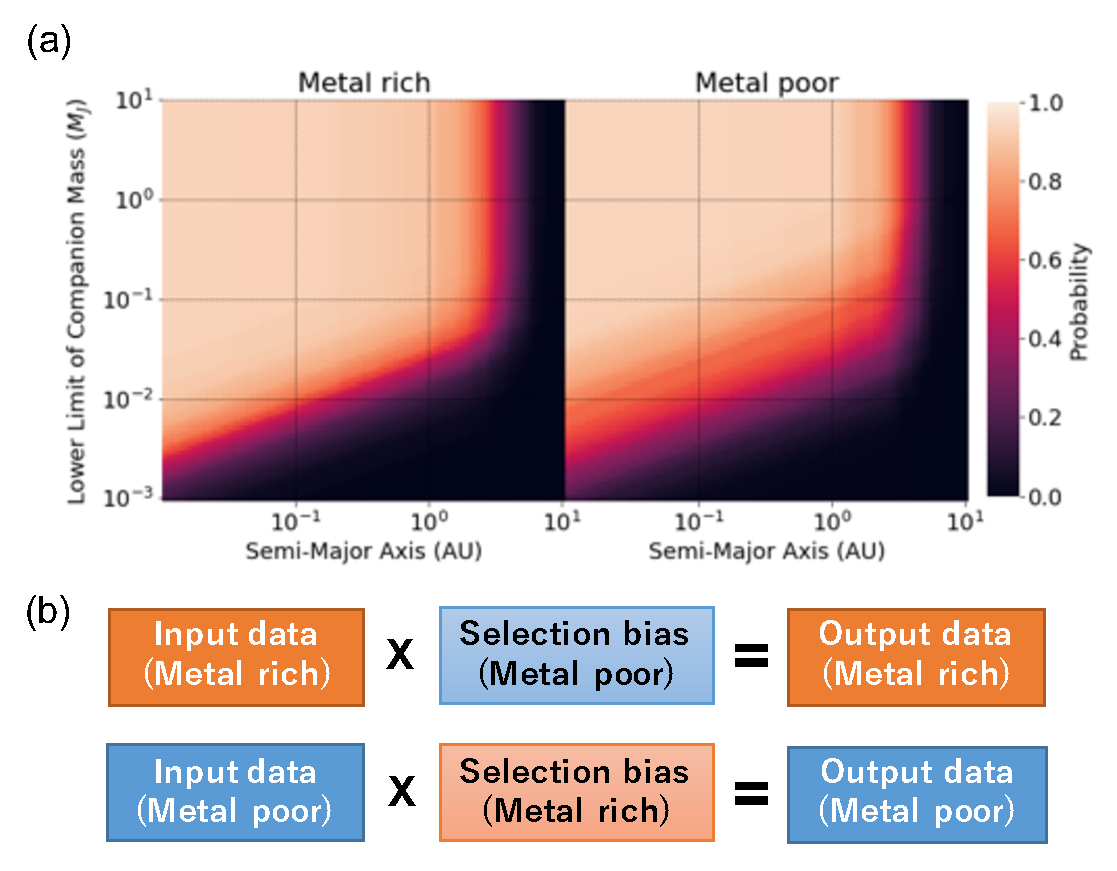
\includegraphics[width=9cm]{../../../Figure/selection_bias.pdf}
\caption{(a) Detectable regions for metal-rich (left) and -poor systems (right). The boundary of metallicity was fixed to 0.0 dex. Each planetary system is observed by the radial velocity measurements with each detection probability. (b) Method for equalizing the two selection biases in two different metallicity regions. The planetary distribution is additionally filtered with the opposite selection bias to remove the different selection biases in the two metallicity regions. \label{fig:bias}}
\end{center}
\end{figure}


\subsection{Preparing Data} \label{subsec:prepare}

The original samples considered in this study are limited to companion objects detected by radial velocity observations, allowing the orbital parameters to be characterized and the lower limit of the companion mass to be determined. Essentially, original samples are selected from those labeled ``Radial Velocity" in the ``detection method" column of the Extrasolar Planet Encyclopedia catalog53 as of the end of June 2018 \citep{2011A&A...532A..79S}. The radial velocities of central stars by orbiting planets, the orbital periods, and eccentricities of planets are also collected from the same catalog. On the other hand, the masses and metallicities of host stars are cited from the SWEET-Cat catalog \citep{2013A&A...556A.150S, 2018A&A...620A..58S}, and the lower limit of companion masses are calculated with Equation (\ref{equ:Mp}). The radii of planets are calculated from the orbital periods and star masses. The metallicities and stellar masses are also extracted from the Casagrande catalog \citep{2011A&A...530A.138C}, the Padova database \citep{2000A&AS..141..371G}, and the BaSTI stellar model \citep{2018ApJ...856..125H}. Then, the correlation between the data from the SWEET-Cat catalog and the others was checked in order to fill up the data lacking of host stars' masses or metallicities with linear conversion. In addition, the measurement accuracies and observation terms for each planetary system as the indicators of selection bias were extracted from exoplanets.org. The observation term and stellar mass supply the upper limit of the maximum semi-major axis of the observable region by the radial velocity measurement for each planetary system. The maximum semi-major axis, the stellar mass and the accuracy of the radial velocity measurement were used for calculation of the lower limit on the mass of the observable planet. The other lacking data is filled up with several studies.

The gaseous objects from all the samples used in this study are extracted in order to remove the impact of low-mass samples, such as Neptune-mass planets (gas dwarfs) and super-Earths, on this analysis. First, we determined the boundary mass between the gaseous and gas-dwarf objects from a perspective of both theory and observation. According to a previous study \citep{2004ApJ...604..388I}, gas-dwarf objects, which primarily consist of heavy-core objects such as Neptune and Uranus, have the potential to grow to the extent allowed by the core building materials inside their semi-major axes. This growth occurs via giant impacts in the inner region of the disk after the disk gas dissipates. However, this core growth is limited by the scattering effect of the heavy core increasing with greater distances from the central star. Therefore, the mass of a gas-dwarf object reaches a maximum at the semi-major axis, where the scattering effect begins to limit the core growth. A boundary between gas giants and gas dwarfs at four times the Earth's radius has been observationally revealed by the Kepler data \citep{2012Natur.486..375B}. From the empirical planetary mass-radius relation \citep{2017A&A...604A..83B}:
\begin{equation}
\frac{R_p}{R_\oplus} \propto \frac{M_p}{M_\oplus}\pm0.02 ,
\end{equation}
we found that the boundary of planetary mass is about 30 times the Earth's mass, which is equal to 0.1 $\rm M_J$. Note that \cite{2004ApJ...604..388I} also indicates that the boundary of planetary mass is 0.1 $\rm M_J$. Based on these considerations, 0.1 $\rm M_J$ is applied in this study as the boundary mass between gas giants and gas dwarfs. Performing these preprocessing for all data observed by radial velocity observations, we use 520 planetary systems and 623 planets in this study.


\subsection{Analysis Method} \label{analysis}

As shown previous section, core-accretion and disk-instability processes are likely to depend on the disk metallicity. Then, we investigate whether the distributions of planet mass or orbital parameters of the common-biased samples, which are minimized the difference of the selection effects depending on the metallicity, differ by the metallicity regions with the AD test. We determine the metallicity that divides the common-biased samples into two regions as ``metallicity boundary," and derive the p-values of the AD test for the distributions of planet mass and semi-major axis in the higher/lower metallicity regions than the metallicity boundary. Changing the metallicity boundary, we fix the boundary with the lowest p-value. We show how different the distributions of two common-biased sub-samples are when they are divided with the metallicity boundary in next section. Thus, dividing the common-biased samples with the metallicity boundary, we compare the distributions of the semi-major axis and planet mass in each metallicity region, and confirm whether the distributions are different. This result is shown in Section \ref{subsec:metal}. Next, we investigate whether the planetary distribution, whose selection effect is equalized by the metallicity, is classified into two regimes with GMM as previous study. We also verify whether the planet-masse and eccentricity distributions of classified common-biased samples are different.


\section{Results} \label{sec:results}

In this section, we quantitively show how different the distributions of the orbital properties and planet masses for the extrasolar gaseous objects orbiting the metal-rich and -poor regions are, minimizing the impact of the selection effect on their distributions. We also explore how many components exit in the extrasolar gaseous objects through classifying the common-biased samples with the Gaussian Mixture Model (GMM).


\subsection{Two Metallicity Regions} \label{subsec:metal}

We first determined the boundary of metallicity that divides the original samples into two such that the distributions of planet mass and semi-major axis in the two metal-rich and -poor regions are most different, respectively, using the method that considers the selection effects of the radial velocity measurements, as explained in Section 2.1. Figure \ref{fig:pvalue} shows the p-values derived by the two-sample AD test for the distributions of the semi-major axes and lower mass limits of the common-biased samples, changing the boundary of metallicity from -0.7 to 0.4 dex. Note that the common-biased samples, which were applied to the AD test, were constructed such that the impacts of the selection effects in the metal-rich and -poor regions on the common-biased sub-samples are equalized; the comparison between the two distributions of the common-biased sub-samples is not affected by the selection effects of the radial velocity measurements. We iterated the calculation 1,000 times and averaged the calculated p-values for each divided point to derive the mean and standard deviation of the p-values. The minimum p-values of the AD tests for the distributions of the semi-major axis and the planet mass were $2.4\times10^{-3}$ and $3.5\times10^{-5}/4.2\times10^{-5}$ at the metallicity of -0.04 and -0.29/-0.06 dex, respectively; thus, the planetary distributions in the metal-rich and -poor regions do not arise from the selection effect of the radial velocity measurements but from the planet formation and evolution. In this study, we used applied -0.05 dex as the boundary of metallicity through considering that the two minimum p-values are around -0.05 dex.

Next, we compared the distributions of the lower mass limit and semi-major axis for the common-biased sub-samples in the metal-rich and -poor regions that are divided by the boundary of metallicity. Figure \ref{fig:a_Mp} shows two scatter plots of the common-biased sub-samples in the metal-rich and -poor regions on the semi-major axis and lower-mass limit and compared the cumulative fractions of the common-biased sub-samples in terms of the semi-major axis and lower-mass limit, respectively. The gas giants with semi-major axis less than 0.1 au and the planets more massive than about 5 $\rm M_J$ in the metal-poor region are relatively lack and excess compared to those in the metal-rich region, respectively. We discuss where the difference between the planetary distributions in the metal-rich and -poor regions comes from in Section \ref{sec:discussion}.

\begin{figure}[t]
\begin{center}
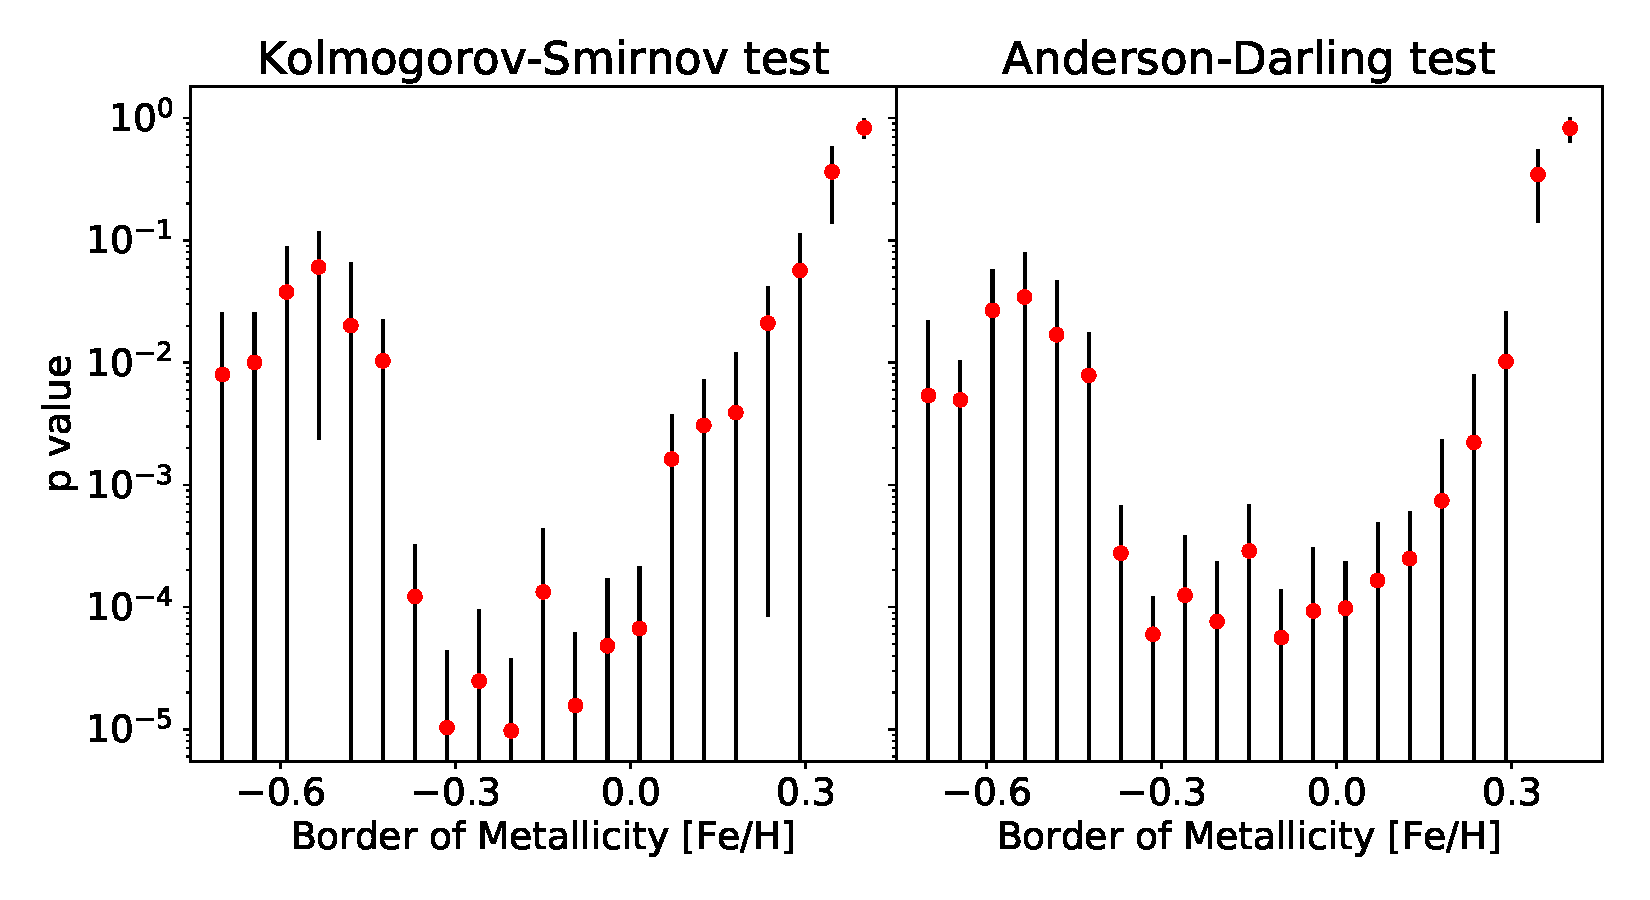
\includegraphics[width=9cm]{../../../Figure/pvalues_plot.pdf}
\caption{P-values of AD test for the semi-major axis (left) and the lower limit on the planet mass (right) of the \red<original> samples as a function of the boundary of metallicity. Red points and black vertical bars are p-values and their standard deviations calculated with 1000 iterations. \label{fig:pvalue}}
\end{center}
\end{figure}

\begin{figure}[t]
\begin{center}
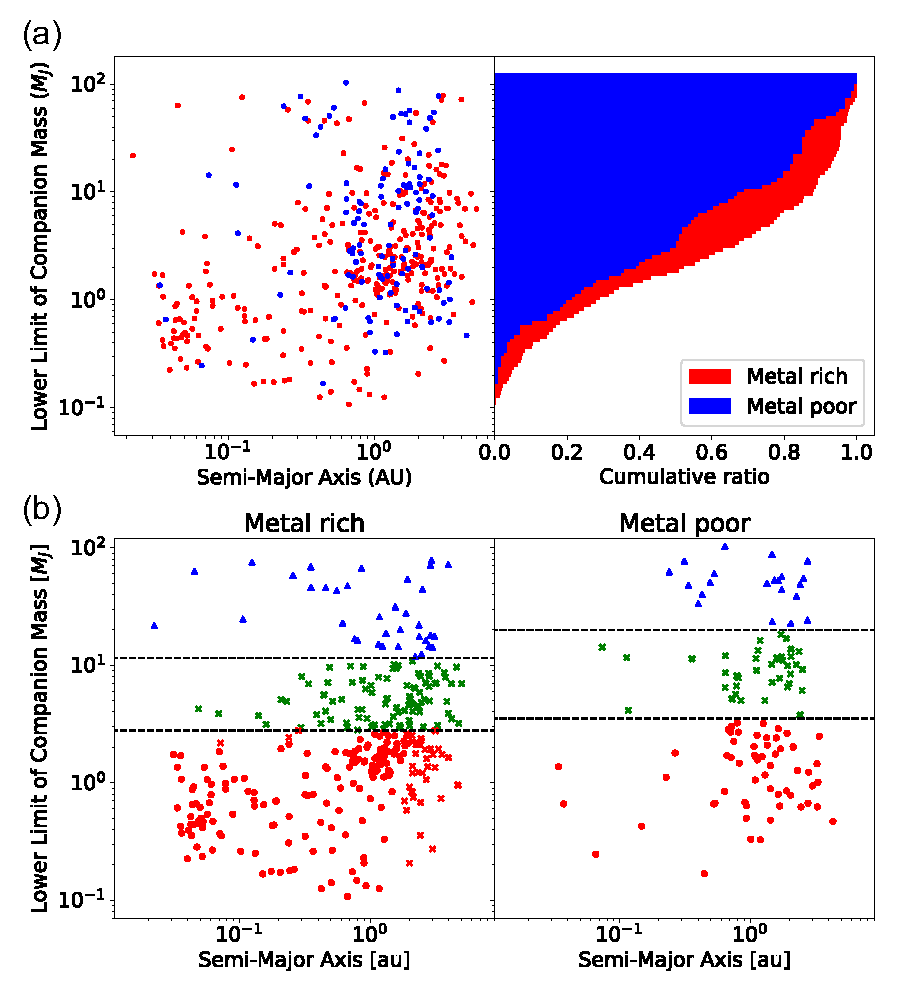
\includegraphics[width=9cm]{../../../Figure/a_Mp.pdf}
\caption{Planetary distributions of the semi-major axes and lower-limit of companion masses for the \red<extracted> samples in the high- and low-metallicity regions (upper left), and cumulative distributions of semi-major axis (bottom) and lower limit of companion mass (right). Red and blue points/bins represent metal-rich and -poor samples, respectively. \label{fig:a_Mp}}
\end{center}
\end{figure}


\subsection{Three Mass-Regimes of Gaseous Objects} \label{subsec:mass}

We classified the 623 common-biased samples into multiple sub-samples on the host-star metallicity and planet-mass plane with the GMM to explore how many sub-samples exist in the extrasolar gas giants discovered to data, given that each sub-sample follow a normal distribution \citep[e.g.,][]{2017A&A...603A..30S, 2018ApJ...853...37S}. Changing the number of the sub-samples, we evaluated each model with the Bayesian Information Criterion (BIC) and found that the three-component model is suitable as the best Gaussian Mixture Model for the 623 common-biased samples. Figure \ref{fig:gmm} shows the best suited model for the common-biased samples. The common-biased samples are divided into three almost along two boundary masses of 4 and 20 $\rm M_J$. The three-component model results from relative paucity of the common-biased samples in two specific regions in the diagram of host-star metallicity versus companion mass; the two regions indicate gaseous objects with masses ranging from 20 to 30 $\rm M_J$ around both the metal-rich and -poor stars and those with masses ranging from 0.1 to 4 $\rm M_J$ around the metal-poor stars. The mean metallicity of the stars hosting the gaseous objects more with masses from 4 to 20 $\rm M_J$ is lower than that of the lighter samples and the mean metallicity of the samples more massive than 20 $\rm M_J$ is much lower than those of the other two sub-samples. Thus, the three-mass regimes exist in the extrasolar gaseous objects discovered so far instead of the two-mass regimes proposed by the previous studies \citep{2007A&A...464..779R, 2017A&A...603A..30S, 2018ApJ...853...37S}. Based on the theoretical studies on the maximum mass of the core-accreted planet \citep[e.g.,][]{2012A&A...541A..97M, 2016ApJ...823...48T}, we redefined the samples lighter than 20 $\rm M_J$ as planetary-mass objects and labeled the two sub-samples with masses from 0.1 to 4 $\rm M_J$ and from 4 to 20 $\rm M_J$ as ‘intermediate-mass planets’ and ‘massive planets.’ In addition, the samples more massive than 20 $\rm M_J$ are labeled as ‘brown dwarfs.’ Note that the boundary between planetary mass and brown dwarf objects established by the deuterium-burning minimum mass of ~ 10 $\rm M_J$ mentioned in a previous study is semantic \citep{2014prpl.conf..619C}; this boundary has no physical meaning from the perspective object evolution.

We next investigated the eccentricity distributions of the brown dwarfs, massive planets, and intermediate-mass planets in both the metal-rich and -poor regions, respectively. The upper panels of Figure \ref{fig:e_Mp} are scatter plots of the common-biased samples in the diagram of eccentricity versus companion mass in the metal-rich and -poor regions. The bottom panels are the cumulative fractions of the eccentricities for the three populations orbiting the metal-rich and -poor stars, respectively. The observational result common to the common-biased samples orbiting the metal-rich and -poor stars is that, while the eccentricities of the brown dwarfs uniformly distribute from 0 to 1, about 80 \% of the intermediate-mass planets have eccentricities smaller than 0.3. In contrast, the eccentricity distributions of the massive planets in the metal-rich and -poor regions are largely different; while the cumulative fraction of the eccentricities for the massive planets orbiting the metal-rich stars is close to that of the brown dwarf, that of the metal-poor massive planets is consistent with that of the intermediate-mass planets. In fact, as shown in Figure \ref{fig:e_ave}, the mean eccentricity of the massive planets decreases as the metallicity of the host star decreases. Thus, the eccentricity distributions also support the three-mass regimes of the extrasolar gaseous objects.

\begin{figure}[t]
\begin{center}
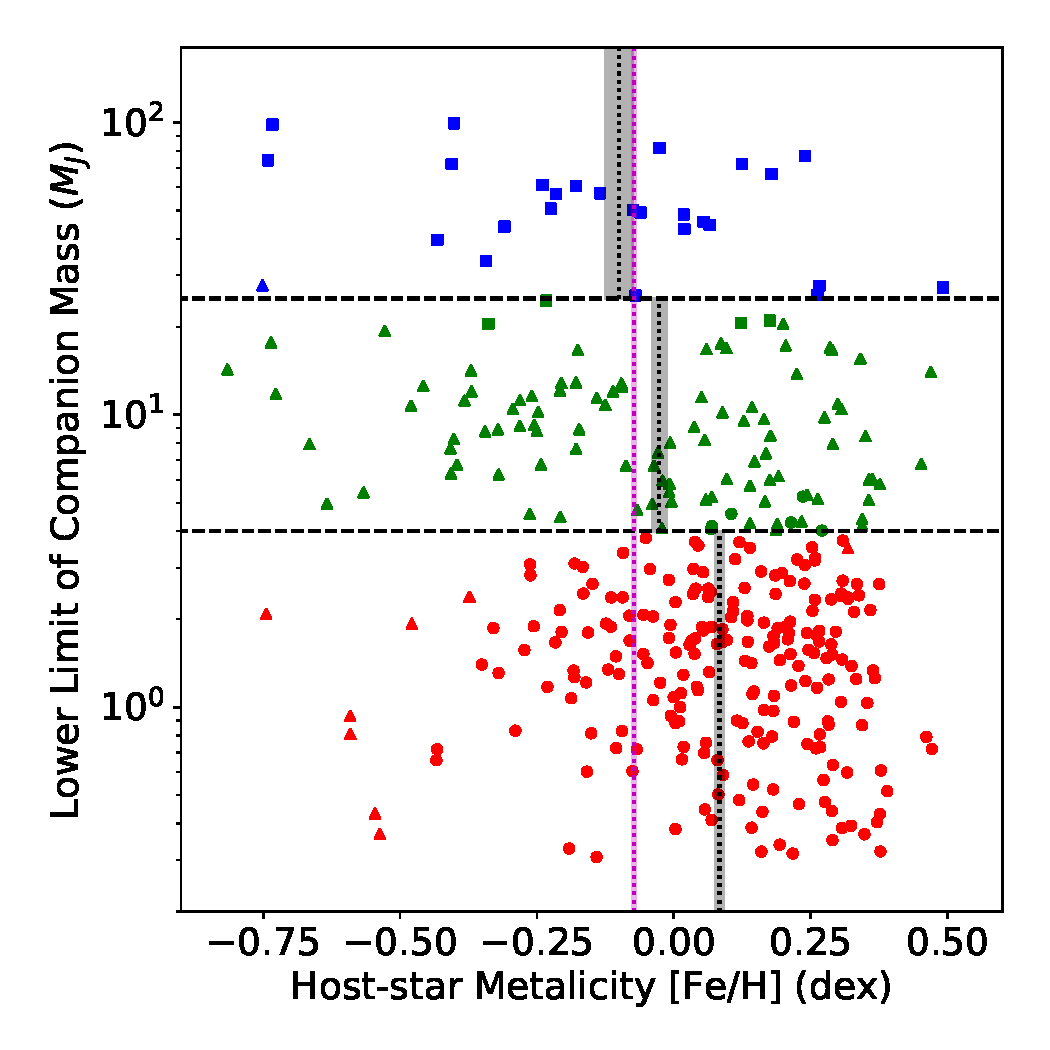
\includegraphics[width=7cm]{../../../Figure/gmm.pdf}
\caption{Distribution classified into three clusters from GMM. The samples of each cluster is described with different markers of square, triangle, and circle. The blue, green, and red points are samples divide into three fields by the mass boundaries (black horizontal lines). The black vertical lines and gray regions are the means and standard errors of metallicity in each field. \label{fig:gmm}}
\end{center}
\end{figure}

\begin{figure}[t]
\begin{center}
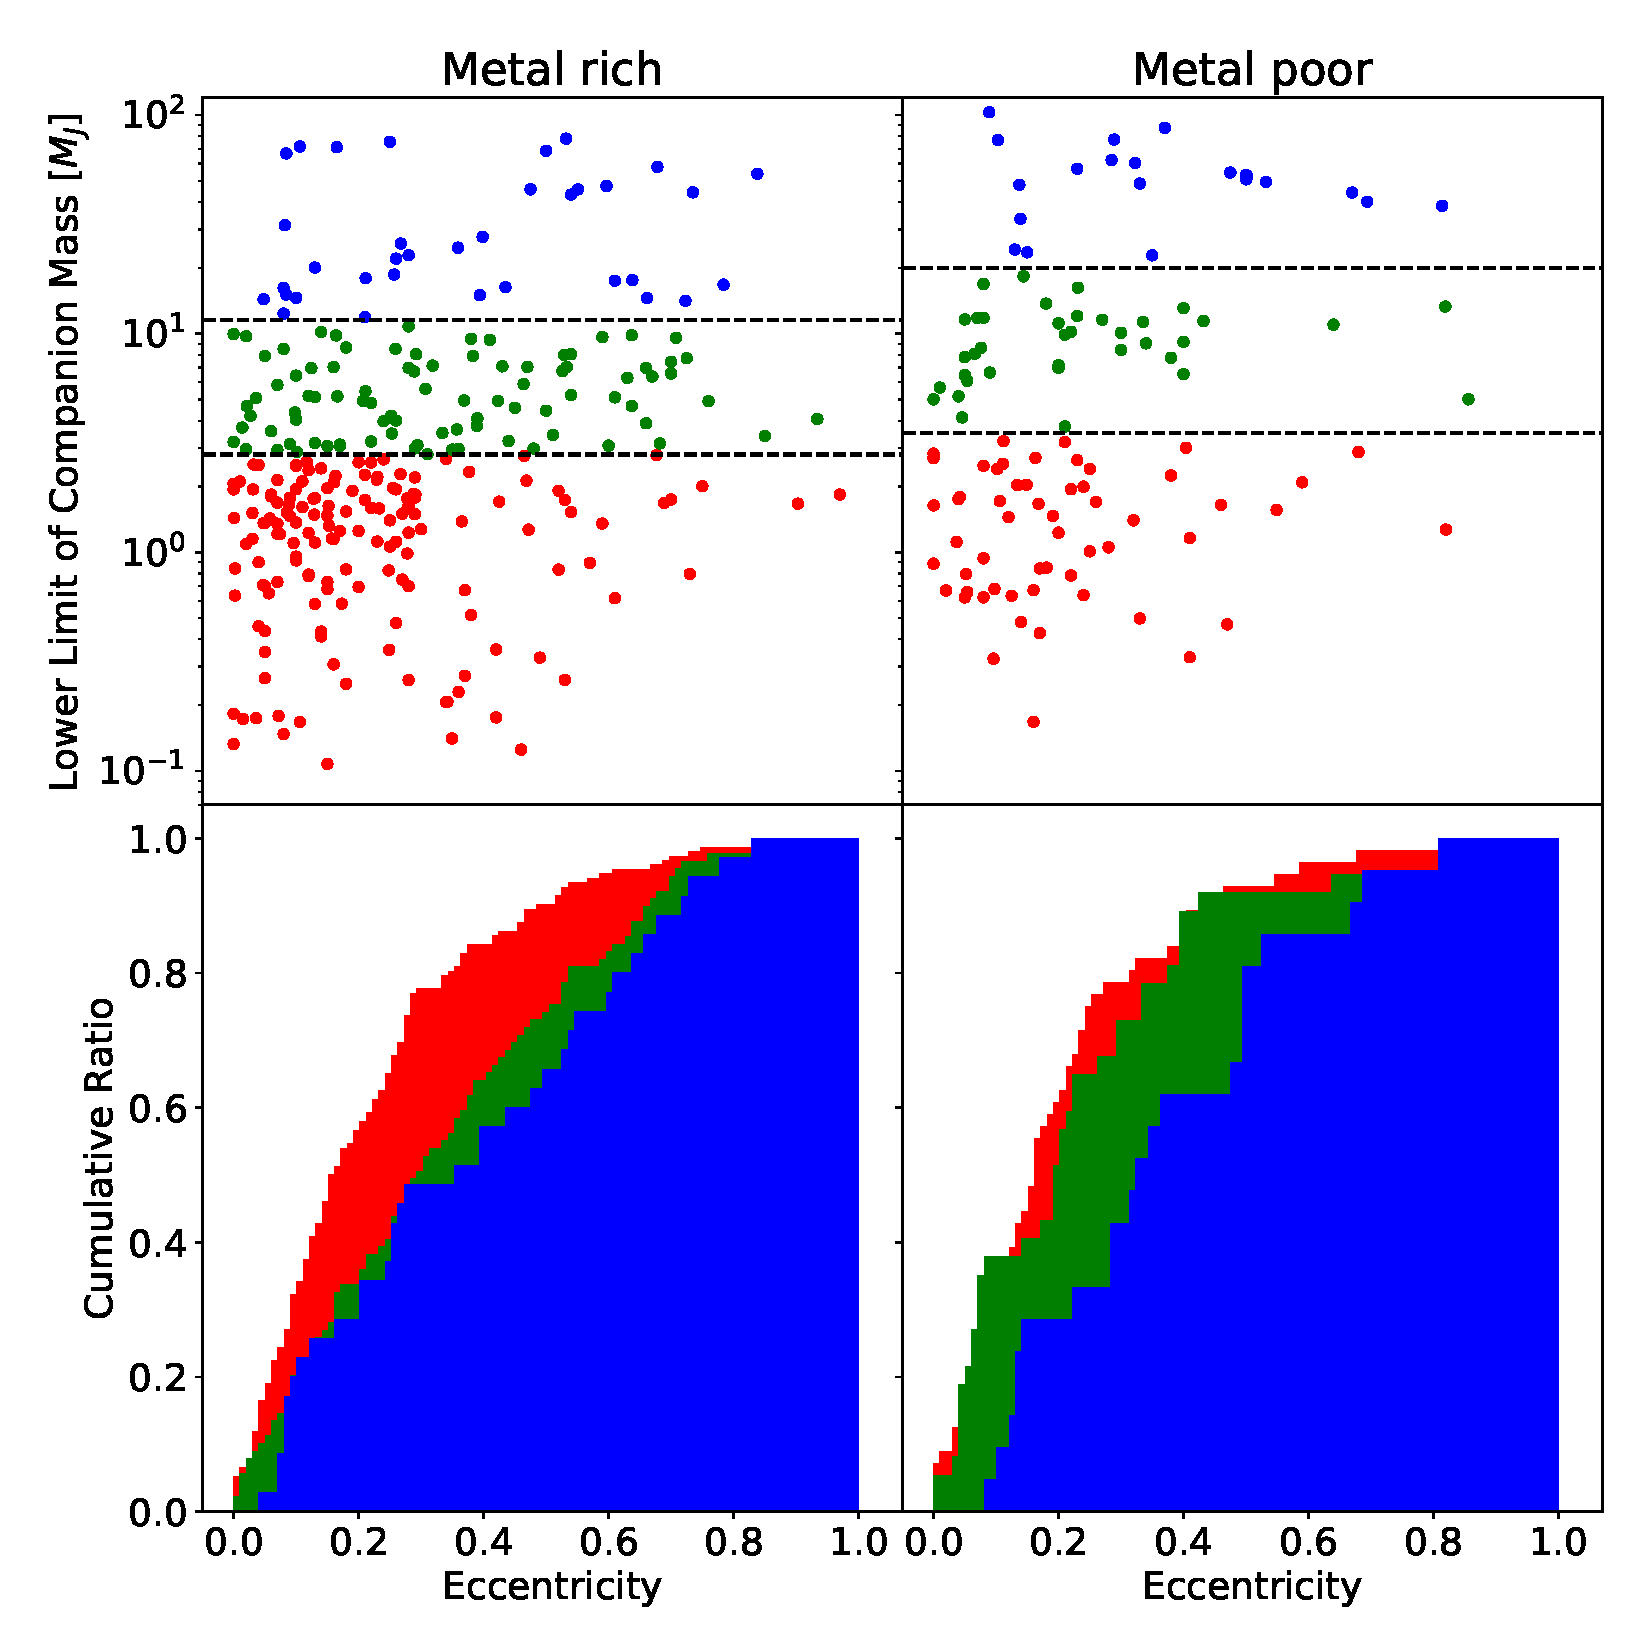
\includegraphics[width=9cm]{../../../Figure/e_Mp_merge.pdf}
\caption{Distributions of the eccentricities and lower limits of companion mass (top) and the cumulative distributions of eccentricities for the gas giants in the metal-rich and -poor regions (bottom). The \red<horizontal lines and> three colors represent the same as those of Figure \ref{fig:gmm}. \red<The white steps show the distributions as uniform.> \label{fig:e_Mp}}
\end{center}
\end{figure}

\begin{figure}[t]
\begin{center}
\includegraphics[width=9cm]{../../../Figure/e_ave.pdf}
\caption{\red<Bins plot of the host-star metallicities and eccentricities. The range of metallicity for each bin is 0.26 (dex), and the red and green bins represent the intermediated and massive planets, respectively. The heights and black vertical bars of each bin are the means and standard errors of the eccentricities included in each range.> \label{fig:e_ave}}
\end{center}
\end{figure}


\section{Discussion} \label{sec:discussion}

In this section, we compare the above results of planetary mass and eccentricity distributions with previous studies and verify the relationship. We also discuss the behavior of planetary distributions in the metal-rich and -poor regions, comparing the observed dataset from the simulation of \cite{2012A&A...541A..97M}.


\subsection{?}

In \cite{2012A&A...541A..97M}, planets are formed by classical core accretion model, and the final semi-major axes and planetary masses are determined, based on the simulation included the planetary migration in disks and the disk evolution. From our study, the two observed planetary-mass distributions, which were divided by the metal boundary, had different expanses. Then, we discuss each planetary-formation process, comparing the distribution of observed data with that of simulation data. Figure \ref{fig:simulation} shows that the comparison between the observed data included the selection biases and simulation data cited from \cite{2012A&A...541A..97M}. The simulation data were also filtered by both selection biases of metal-rich and -poor regions to complete the conditions with the observed data. As the result, the distributions of metal rich regions are very consistence, which can explain that most of gas giants in the metal rich region are formed by core accretion. This is also explained by our results shown in Section \ref{subsec:eccentricity} because of below interpretation. The interaction between a gas giant and protoplanetary disk possibly makes the eccentricity of planet grow \citep{2003ApJ...585.1024G, 2006A&A...447..369K}. This interaction is concentrated at discrete Lindblad and corotation resonances, which causes the planet's orbit to migrate and open a gap in the disk as the planet mass is large enough. If the viscous coefficient equals to $10^{-5}$, the planet with circular orbit changes to eccentric orbit as the planetary mass is over 3 $\rm M_J$. The more massive planets make their eccentricity higher until the maximum value 0.25. On the other hand, if a planetary system has two gas giants, the outer planet may prolong the orbital period of the inner planet. These planets' eccentricities grow up in rough inverse proportion to their masses by this orbital interaction \citep{2002ApJ...564L.105C}. From the verification of simulation \citep{2013ApJ...775...42I}, gas giants and rocky/icy planets emerge, migrate, and undergo dynamical instability in a relatively massive disk, and the perturbation between planets causes orbital crossing, eccentricity excitation, and planetary ejection. Therefore, gas giants formed through core accretion tend to have high eccentricities, which is consistent to our results of eccentricity distribution.

In contrast, the distributions of metal poor regions between the observed data and the simulation data are different. This means that the planetary formation process in metal poor disks differs from in metal rich disks: the planetary formation in metal poor region cannot be explained by only core accretion. On the other hand, the eccentricity of gas giant formed via disk instability ranges from 0 to 0.35 in initial stage, and decreases as the planet mass increases \citep{2011ApJ...731...74B}. Note that the range of semi-major axis is $30\sim70$ au. This trend can be also seen slightly in the metal poor region of Figure \ref{fig:e_Mp}. However, because it is not clear, there possibly exists other formation processes included core accretion in metal poor regions.

\begin{figure}[t]
\begin{center}
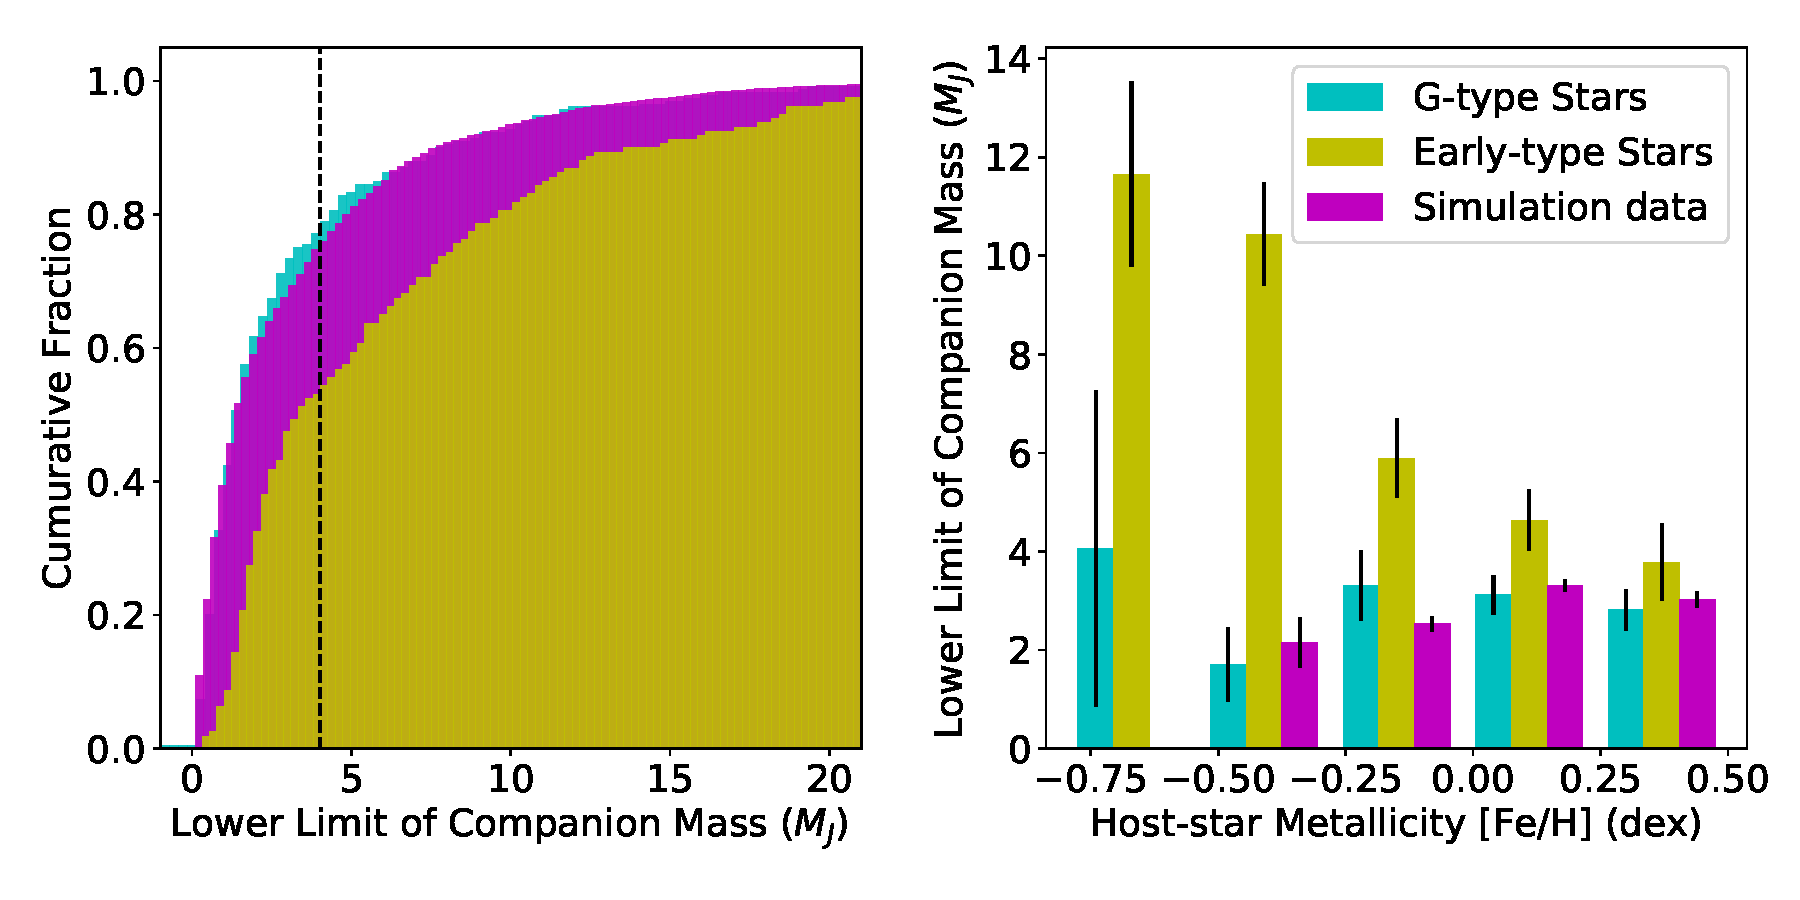
\includegraphics[width=9cm]{../../../Figure/simulation.pdf}
\caption{Comparison of planetary distributions between the observed data (red and blue points) and simulation data (yellow and cyan points) in the metal-rich region (upper left) and the metal-poor region (lower left), and the cumulative maps of planetary masses in the metal-rich region (upper right) and the metal-poor region (lower right). \label{fig:simulation}}
\end{center}
\end{figure}


\subsection{?}

According to previous studies, the planetary distributions are divided into two regions. Host stars over 4 $M_J$ tend to be more metal poor and massive, but below this value show the well-known metallicity-giant planet frequency correlation \citep{2017A&A...603A..30S}. In addition, planets formed through core accretion have upper bound of mass, which equals around 10 $M_J$, and planets over this value likely formed through gravitational disk instability \citep{2018ApJ...853...37S}.  However, we show that the planetary distribution has multiple regions depending on planetary mass and disk metallicity. Figure \ref{fig:metal_Mp} shows that the planetary distribution used in this study. The colors of red and blue mean the planets in metal rich and poor regions, respectively. The markers describe the different ranges of planet mass, which divided with mass boundary determined by the classification in Section \ref{subsec:mass}. 

\textcolor{green}{According to previous studies, the distribution of gas-giant masses can be divided into two regions by the border of 4 $\rm M_J$ with metallicity bias, which insists that the planetary-formation processes in each region are different \citep[e.g.,][]{2017A&A...603A..30S}. In contrast, the boundaries were drawn at 4 and 20 $\rm M_J$ from our result, which the former is consistent with the previous studies. The latter indicates the border between the gas giants and brawn dwarfs.}

\begin{figure*}[t]
\begin{center}
\includegraphics[width=15cm]{../../../Figure/metal_Mp.pdf}
\caption{\label{fig:metal_Mp}}
\end{center}
\end{figure*}


\acknowledgments


\vspace{5mm}


\begin{thebibliography}{}

\bibitem[Adibekyan et al.(2013)]{2013A&A...560A..51A} Adibekyan, V.~Z., Figueira, P., Santos, N.~C., et al.\ 2013, \aap, 560, A51
\bibitem[Bashi et al.(2017)]{2017A&A...604A..83B} Bashi, D., Helled, R., Zucker, S., \& Mordasini, C.\ 2017, \aap, 604, A83
\bibitem[Boss(1997)]{1997Sci...276.1836B} Boss, A.~P.\ 1997, Science, 276, 1836
\bibitem[Boss(2002)]{2002ApJ...567L.149B} Boss, A.~P.\ 2002, \apjl, 567, L149
\bibitem[Boss(2011)]{2011ApJ...731...74B} Boss, A.~P.\ 2011, \apj, 731, 74
\bibitem[Buchhave et al.(2012)]{2012Natur.486..375B} Buchhave, L.~A., Latham, D.~W., Johansen, A., et al.\ 2012, \nat, 486, 375
\bibitem[Cai et al.(2006)]{2006ApJ...636L.149C} Cai, K., Durisen, R.~H., Michael, S., et al.\ 2006, \apjl, 636, L149
\bibitem[Casagrande et al.(2011)]{2011A&A...530A.138C} Casagrande, L., Sch{\"o}nrich, R., Asplund, M., et al.\ 2011, \aap, 530, A138
\bibitem[Chabrier et al.(2014)]{2014prpl.conf..619C} Chabrier, G., Johansen, A., Janson, M., \& Rafikov, R.\ 2014, Protostars and Planets VI, 619
\bibitem[Chiang et al.(2002)]{2002ApJ...564L.105C} Chiang, E.~I., Fischer, D., \& Thommes, E.\ 2002, \apjl, 564, L105
\bibitem[Dawson \& Murray-Clay(2013)]{2013ApJ...767L..24D} Dawson, R.~I., \& Murray-Clay, R.~A.\ 2013, \apjl, 767, L24
\bibitem[Dodson-Robinson et al.(2009)]{2009ApJ...707...79D} Dodson-Robinson, S.~E., Veras, D., Ford, E.~B., \& Beichman, C.~A.\ 2009, \apj, 707, 79
\bibitem[Dupuy \& Liu(2011)]{2011ApJ...733..122D} Dupuy, T.~J., \& Liu, M.~C.\ 2011, \apj, 733, 122
\bibitem[Durisen et al.(2007)]{2007Arizona} Durisen, R. H., Reipurth, V. Jewitt, Keil, K., et al.\ 2007, Univ. of Arizona Press, Tucson 951, 607-622
\bibitem[Fischer \& Valenti(2005)]{2005ApJ...622.1102F} Fischer, D.~A., \& Valenti, J.\ 2005, \apj, 622, 1102
\bibitem[Girardi et al.(2000)]{2000A&AS..141..371G} Girardi, L., Bressan, A., Bertelli, G., \& Chiosi, C.\ 2000, \aaps, 141, 371
\bibitem[Goldreich \& Sari(2003)]{2003ApJ...585.1024G} Goldreich, P., \& Sari, R.\ 2003, \apj, 585, 1024
\bibitem[Hayashi et al.(1985)]{1985prpl.conf.1100H} Hayashi, C., Nakazawa, K., \& Nakagawa, Y.\ 1985, Protostars and Planets II, 1100
\bibitem[Hidalgo et al.(2018)]{2018ApJ...856..125H} Hidalgo, S.~L., Pietrinferni, A., Cassisi, S., et al.\ 2018, \apj, 856, 125
\bibitem[Ida \& Lin($2004a$)]{2004ApJ...604..388I} Ida, S., \& Lin, D.~N.~C.\ 2004a, \apj, 604, 388
\bibitem[Ida \& Lin($2004b$)]{2004ApJ...616..567I} Ida, S., \& Lin, D.~N.~C.\ 2004b, \apj, 616, 567
\bibitem[Ida et al.(2013)]{2013ApJ...775...42I} Ida, S., Lin, D.~N.~C., \& Nagasawa, M.\ 2013, \apj, 775, 42
\bibitem[Kalas et al.(2008)]{2008Sci...322.1345K} Kalas, P., Graham, J.~R., Chiang, E., et al.\ 2008, Science, 322, 1345
\bibitem[Kley \& Dirksen(2006)]{2006A&A...447..369K} Kley, W., \& Dirksen, G.\ 2006, \aap, 447, 369
\bibitem[Kuiper(1951)]{1951PNAS...37....1K} Kuiper, G.~P.\ 1951, Proceedings of the National Academy of Science, 37, 1
\bibitem[Lagrange et al.(2010)]{2010Sci...329...57L} Lagrange, A.-M., Bonnefoy, M., Chauvin, G., et al.\ 2010, Science, 329, 57
\bibitem[Lambrechts \& Johansen(2012)]{2012A&A...544A..32L} Lambrechts, M., \& Johansen, A.\ 2012, \aap, 544, A32
\bibitem[Lee et al.(2012)]{2012MNRAS.424.2832L} Lee, K.~J., Guillemot, L., Yue, Y.~L., Kramer, M., \& Champion, D.~J.\ 2012, \mnras, 424, 2832
\bibitem[Ma \& Ge(2014)]{2014MNRAS.439.2781M} Ma, B., \& Ge, J.\ 2014, \mnras, 439, 2781
\bibitem[Marois et al.(2008)]{2008Sci...322.1348M} Marois, C., Macintosh, B., Barman, T., et al.\ 2008, Science, 322, 1348
\bibitem[Matsuo et al.(2007)]{2007ApJ...662.1282M} Matsuo, T., Shibai, H., Ootsubo, T., \& Tamura, M.\ 2007, \apj, 662, 1282
\bibitem[Mayor \& Queloz(1995)]{1995Natur.378..355M} Mayor, M., \& Queloz, D.\ 1995, \nat, 378, 355
\bibitem[Mayer et al.(2002)]{2002Sci...298.1756M} Mayer, L., Quinn, T., Wadsley, J., \& Stadel, J.\ 2002, Science, 298, 1756
\bibitem[Mayer et al.(2007)]{2007ApJ...661L..77M} Mayer, L., Lufkin, G., Quinn, T., \& Wadsley, J.\ 2007, \apjl, 661, L77
\bibitem[Mayor et al.(2011)]{2011arXiv1109.2497M} Mayor, M., Marmier, M., Lovis, C., et al.\ 2011, arXiv:1109.2497
\bibitem[Mizuno(1980)]{1980PThPh..64..544M} Mizuno, H.\ 1980, Progress of Theoretical Physics, 64, 544
\bibitem[Mordasini et al.(2009)]{2009A&A...501.1161M} Mordasini, C., Alibert, Y., Benz, W., \& Naef, D.\ 2009, \aap, 501, 1161
\bibitem[Mordasini et al.(2012)]{2012A&A...541A..97M} Mordasini, C., Alibert, Y., Benz, W., Klahr, H., \& Henning, T.\ 2012, \aap, 541, A97
\bibitem[Ormel \& Klahr(2010)]{2010A&A...520A..43O} Ormel, C.~W., \& Klahr, H.~H.\ 2010, \aap, 520, A43
\bibitem[Perri \& Cameron(1974)]{1974Icar...22..416P} Perri, F., \& Cameron, A.~G.~W.\ 1974, \icarus, 22, 416
\bibitem[Pollack et al.(1996)]{1996Icar..124...62P} Pollack, J.~B., Hubickyj, O., Bodenheimer, P., et al.\ 1996, \icarus, 124, 62
\bibitem[Ribas \& Miralda-Escud{\'e}(2007)]{2007A&A...464..779R} Ribas, I., \& Miralda-Escud{\'e}, J.\ 2007, \aap, 464, 779
\bibitem[Santos et al.(2003)]{2003A&A...398..363S} Santos, N.~C., Israelian, G., Mayor, M., Rebolo, R., \& Udry, S.\ 2003, \aap, 398, 363
\bibitem[Santos et al.(2004)]{2004A&A...415.1153S} Santos, N.~C., Israelian, G., \& Mayor, M.\ 2004, \aap, 415, 1153
\bibitem[Santos et al.(2013)]{2013A&A...556A.150S} Santos, N.~C., Sousa, S.~G., Mortier, A., et al.\ 2013, \aap, 556, A150
\bibitem[Santos et al.(2017)]{2017A&A...603A..30S} Santos, N.~C., Adibekyan, V., Figueira, P., et al.\ 2017, \aap, 603, A30
\bibitem[Schlaufman(2018)]{2018ApJ...853...37S} Schlaufman, K.~C.\ 2018, \apj, 853, 37
\bibitem[Schneider et al.(2011)]{2011A&A...532A..79S} Schneider, J., Dedieu, C., Le Sidaner, P., Savalle, R., \& Zolotukhin, I.\ 2011, \aap, 532, A79
\bibitem[Sousa et al.(2008)]{2008A&A...487..373S} Sousa, S.~G., Santos, N.~C., Mayor, M., et al.\ 2008, \aap, 487, 373
\bibitem[Sousa et al.(2018)]{2018A&A...620A..58S} Sousa, S.~G., Adibekyan, V., Delgado-Mena, E., et al.\ 2018, \aap, 620, A58
\bibitem[Tanigawa \& Ikoma(2007)]{2007ApJ...667..557T} Tanigawa, T., \& Ikoma, M.\ 2007, \apj, 667, 557
\bibitem[Tanigawa \& Tanaka(2016)]{2016ApJ...823...48T} Tanigawa, T., \& Tanaka, H.\ 2016, \apj, 823, 48
\bibitem[Torres et al.(2008)]{2008ApJ...677.1324T} Torres, G., Winn, J.~N., \& Holman, M.~J.\ 2008, \apj, 677, 1324
\bibitem[Wang \& Fischer(2015)]{2015AJ....149...14W} Wang, J., \& Fischer, D.~A.\ 2015, \aj, 149, 14

\end{thebibliography}

%\appendix

\end{CJK*}
\end{document}
